\documentclass[11pt]{article}

\usepackage[margin=1in]{geometry}
\usepackage[T1]{fontenc}
\usepackage[utf8]{inputenc}
\usepackage{lmodern}
\usepackage{microtype}
\usepackage{amsmath}
\usepackage{amssymb}
\usepackage{booktabs}
\usepackage{hyperref}
\usepackage{enumitem}
\usepackage{xcolor}
\usepackage{graphicx}

\graphicspath{{figures/}}

\hypersetup{
  colorlinks=true,
  linkcolor=blue!50!black,
  urlcolor=blue!50!black,
  citecolor=blue!50!black
}

\title{Deterministic Hermetic Fixture Validation for Throat-Like Transport in Overspace Ray-Tracing Systems}
\author{Project Draft}
\date{April 2026}

\begin{document}
\maketitle

\begin{abstract}
We present a deterministic renderer-validation framework for throat-like transport behavior in overspace ray-tracing systems. The framework promotes selected overspace scenes into hermetically enclosed fixtures and evaluates them through the \texttt{GrinFilmCamera} transport path rather than through interactive rasterized inspection alone. Within this harness, every pixel is required to return a classified transport outcome within the configured transport budget. The current taxonomy includes \texttt{geom\_hit}, \texttt{portal\_hit}, \texttt{throat\_entry}, \texttt{throat\_exit}, \texttt{throat\_shell\_transform}, \texttt{throat\_inner\_absorb}, \texttt{background\_hit}, \texttt{escaped\_no\_hit}, and \texttt{budget\_exhausted}. In the current sealed fixture we obtain full-frame classified pixel coverage with deterministic artifact generation, including category maps, legends, summary reports, and a throat-depth interaction map. The current scope is intentionally narrower than full Einstein or Morris--Thorne metric transport; the contribution is a validation-first renderer framework and throat-transport taxonomy that can support later, stronger transport models.
\end{abstract}

\section{Introduction}
Portal and wormhole-inspired rendering demos can show compelling traversal behavior without yet establishing that the renderer can account for every pixel outcome in a sealed scene. That distinction matters once the system is used as a research instrument rather than only as a visual demo. A transport system that leaves rays effectively unaccounted for may still look plausible, but it is weaker as a validation substrate.

This paper frames the current overspace work as a deterministic renderer-validation framework. The focus is not to claim a physically complete wormhole solution. Instead, the goal is to show that throat-like transport can be studied in a controlled, hermetic fixture where every pixel is classified, every run is reproducible, and failure states remain visible rather than hidden.

\section{Related Framing and Positioning}
The present work sits between two familiar modes. On one side are game-engine and portal-style rendering systems, where traversal and spatial remap are implemented for interactivity and continuity. On the other side are lensing and wormhole transport models, where the transport law itself becomes the subject of interpretation.

The present contribution is neither a new analytic solution nor a claim of completed general-relativistic rendering. The contribution is a validation language built around hermetic fixtures, explicit transport categories, deterministic capture, and renderer-side evidence that all pixels resolve to classified outcomes.

\section{System Architecture}
The current implementation has four layers:
\begin{enumerate}[leftmargin=1.5em]
\item an additive throat-aware portal seam that preserves the stable portal transport shell,
\item a hermetic overspace fixture rendered through \texttt{GrinFilmCamera},
\item renderer-side per-pixel transport classification, and
\item a deterministic artifact pipeline that writes machine-readable and human-readable outputs.
\end{enumerate}

The validated fixture path used in this draft is:
\begin{itemize}[leftmargin=1.5em]
\item scene: \texttt{res://test-overspace-hermetic-fixture.tscn}
\item launcher: \texttt{./scripts/run\_fixture\_005.sh}
\item run directory: \texttt{output/fixture\_005/2026-04-13T22-57-53}
\end{itemize}

\section{Hermetic Fixture Rule}
For enclosed overspace validation scenes we adopt the following harness rule:

\begin{quote}
A scene promoted to an overspace validation fixture should be hermetically enclosed and should produce 100\% classified pixel outcomes under \texttt{GrinFilmCamera} transport, within the configured transport budget.
\end{quote}

This is a validation rule rather than a universal physical law. Its purpose is methodological: if a pixel is not classified, the harness should expose that gap rather than hide it behind visually plausible output.

For a hermetic enclosed fixture, the primary contracts are:
\begin{align*}
\texttt{classified\_pixels} &= \texttt{total\_pixels} \\
\texttt{classified\_coverage\_ratio} &= 1 \\
\texttt{escaped\_no\_hit} &\approx 0 \\
\texttt{budget\_exhausted} &\approx 0
\end{align*}

\section{Throat Taxonomy}
The current taxonomy should be read as a renderer-facing causal vocabulary:
\begin{itemize}[leftmargin=1.5em]
\item \texttt{geom\_hit}: final classified outcome lands on explicit scene geometry,
\item \texttt{portal\_hit}: outcome is attributable to the portal seam without a richer throat-shell event,
\item \texttt{throat\_entry}: entry-side boundary-layer event at the throat,
\item \texttt{throat\_exit}: exit-side boundary-layer event at the throat,
\item \texttt{throat\_shell\_transform}: shell-mediated transformation in the current bounded throat model,
\item \texttt{throat\_inner\_absorb}: terminal absorption in the current inner-throat model,
\item \texttt{background\_hit}: intentional background classification when present,
\item \texttt{escaped\_no\_hit}: transport escaped classification before termination,
\item \texttt{budget\_exhausted}: transport budget ended before classification completed.
\end{itemize}

An aggregate summary count is preserved:
\[
\texttt{throat\_event} = \texttt{throat\_entry} + \texttt{throat\_exit} + \texttt{throat\_shell\_transform} + \texttt{throat\_inner\_absorb}.
\]

\section{Deterministic Validation Method}
The current deterministic validation method is:
\begin{enumerate}[leftmargin=1.5em]
\item build the active WSL repository,
\item launch the hermetic fixture through \texttt{fixture\_005},
\item capture renderer-side transport classification and debug imagery,
\item parse the raw run log into deterministic reports and image artifacts,
\item verify the hermetic coverage invariant from the emitted metrics.
\end{enumerate}

The current additional diagnostic layer is a throat-depth map. This map records per-pixel throat interaction count derived from current renderer state and emits dedicated image, legend, and JSON/TXT artifacts.

\section{Current Results}
The evidence base for this draft is the validated \texttt{fixture\_005} run at \texttt{2026-04-13T22-57-53}. Table~\ref{tab:results} summarizes the current metrics.

\begin{table}[h]
\centering
\begin{tabular}{lr}
\toprule
Metric & Value \\
\midrule
Total pixels & 129600 \\
Classified pixels & 129600 \\
Classified coverage ratio & 1.0 \\
Escaped no-hit & 0 \\
Budget exhausted & 0 \\
Unclassified & 0 \\
Geom hit & 75387 \\
Portal hit & 32374 \\
Throat event & 21839 \\
Throat entry & 0 \\
Throat exit & 132 \\
Throat shell transform & 21707 \\
Throat inner absorb & 0 \\
Throat pixels & 33356 \\
Max interaction count & 107 \\
Mean interaction count & 2.364102 \\
\bottomrule
\end{tabular}
\caption{Validated \texttt{fixture\_005} results, run \texttt{2026-04-13T22-57-53}.}
\label{tab:results}
\end{table}

\begin{figure}[h]
\centering

\includegraphics[width=0.48\textwidth]{capture.png}
\hfill
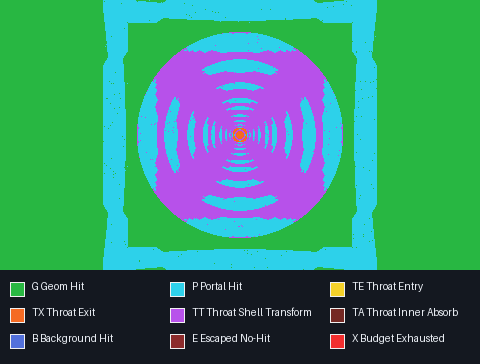
\includegraphics[width=0.48\textwidth]{coverage_annotated.png}
\caption{Left: raw transport capture. Right: per-pixel transport category overlay.}
\label{fig:coverage}
\end{figure}

\begin{figure}[h]
\centering

\includegraphics[width=0.48\textwidth]{throat_depth_map.png}
\hfill
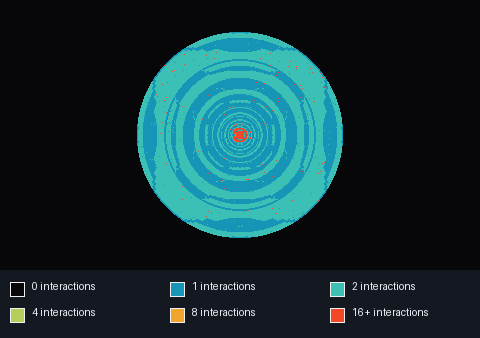
\includegraphics[width=0.48\textwidth]{throat_depth_annotated.png}
\caption{Left: throat interaction depth map. Right: annotated depth map with legend.}
\label{fig:throat}
\end{figure}

\section{Limitations}
The current system has clear limits:
\begin{itemize}[leftmargin=1.5em]
\item it is not full Einstein or Morris--Thorne metric transport,
\item it does not solve the Einstein field equations,
\item it does not claim a physically complete relativistic wormhole renderer,
\item the current throat semantics are bounded framework semantics layered over a stable portal seam.
\end{itemize}

The framework is therefore stronger than a visual portal demo but weaker than a complete relativistic transport model.

\section{Future Work}
The next technically natural steps are:
\begin{enumerate}[leftmargin=1.5em]
\item richer \texttt{BoundaryLayerVolume} attribution for shell behavior,
\item entry and exit symmetry refinement without destabilizing the fixture,
\item additional hermetic fixtures with different throat geometries and camera placements,
\item later integration with stronger curvature-aware or metric-aware transport models.
\end{enumerate}

\section{Reproducibility Appendix}
Commands used for the current milestone:

\begin{verbatim}
cd /home/bb/code/godot_xPRIMEray
dotnet build 'Physical Light and Camera Units.csproj' -c Debug -v minimal
python3 -m py_compile tools/fixture_characterization_report.py tools/fixture_005_report.py
./scripts/run_fixture_005.sh
\end{verbatim}

Direct report regeneration:

\begin{verbatim}
.venv/bin/python tools/fixture_005_report.py \
  --fixture-id fixture_005 \
  --timestamp 2026-04-13T22-57-53 \
  --scene res://test-overspace-hermetic-fixture.tscn \
  --launcher run_fixture_005 \
  --run-dir output/fixture_runs/fixture_005/2026-04-13T22-57-53 \
  --log-path output/fixture_runs/fixture_005/2026-04-13T22-57-53/run.log \
  --capture-path output/fixture_runs/fixture_005/2026-04-13T22-57-53/capture.png \
  --runtime-seconds 17.799335 \
  --godot-exit-code 0 \
  --settle-frames 12 \
  --min-rh-step 1 \
  --min-processed-rows 270 \
  --capture-film-opacity 1.0 \
  --compare-grid 0 \
  --compare-crosshair 0 \
  --requested-step-length 0.05 \
  --requested-min-step-length 0.02 \
  --requested-steps-per-ray 640 \
  --requested-turn-threshold 2.4 \
  --requested-error-tolerance 0.010
\end{verbatim}

\end{document}
